\documentclass[11pt,letterpaper]{article}
\usepackage[utf8]{inputenc}
\usepackage[T1]{fontenc}
\usepackage[spanish,es-tabla,es-noshorthands]{babel}
\usepackage[margin=2.25cm]{geometry}
\usepackage{mathptmx}
\usepackage{amsmath}
\usepackage{xcolor}
\usepackage{graphicx}
\usepackage{booktabs}
\usepackage{multirow}
\usepackage{float}
\usepackage{caption}
\usepackage[colorlinks=true,linkcolor=blue!55!black,citecolor=blue!55!black,urlcolor=blue!55!black]{hyperref}
\usepackage{titlesec}
\usepackage{enumitem}

\graphicspath{{../output/figuras/}}
\captionsetup{font=small,labelfont=bf,skip=4pt}
\titlespacing*{\section}{0pt}{8pt}{3.5pt}
\titlespacing*{\subsection}{0pt}{6pt}{2.5pt}
\titleformat*{\section}{\large\bfseries}
\titleformat*{\subsection}{\normalsize\bfseries}
\setlength{\parskip}{2.2pt}
\setlist{nosep,leftmargin=1.35em}

\title{Integración del efecto de las soluciones \emph{Behind-the-Meter} en las
prácticas de estimación de demanda a largo plazo del sistema eléctrico colombiano}
\date{}

\begin{document}

% ============================================================ PORTADA
\begin{titlepage}
\centering
{\scshape Universidad de los Andes\\ Departamento de Ingeniería Eléctrica y Electrónica\par}
\vspace{0.6cm}
{ILE4100, Planeamiento de Sistemas de Potencia\par Proyecto 1\par}
\vspace{2.0cm}
{\Large\bfseries Integración del efecto de las soluciones \emph{Behind-the-Meter} (BtM)
en las prácticas de estimación de demanda a largo plazo del sistema eléctrico
colombiano\par}
\vspace{0.7cm}
{\itshape Propuesta metodológica y validación empírica con modelos multivariados
(VAR/VEC y panel) sobre datos históricos de Colombia y España, ajuste de las
proyecciones UPME 2026-2040 y análisis del umbral del 4\,\% de la CREG\par}
\vspace{2.2cm}
\begin{tabular}{c}
\textbf{Tomas Castro Roa}\\[2pt] \rule{6cm}{0.4pt}\\ {\small Firma}\\[15pt]
\textbf{William David Velasquez Baron}\\[2pt] \rule{6cm}{0.4pt}\\ {\small Firma}\\[15pt]
\textbf{Carlos Fernando Diaz Vargas}\\[2pt] \rule{6cm}{0.4pt}\\ {\small Firma}\\
\end{tabular}
\vfill
{Bogotá D.C., agosto de 2026\par}
\end{titlepage}

% ============================================================ RESUMEN
\noindent\textbf{Resumen.}
Las soluciones \emph{Behind-the-Meter} (BtM) reducen la demanda que registra el
operador sin reducir el consumo real de electricidad, de modo que las series
sobre las que se estiman los modelos oficiales de proyección quedan
progresivamente ``enmascaradas''. Este trabajo propone y \emph{valida
empíricamente} una metodología de cuatro pasos para incorporar dicho efecto en
la práctica colombiana de estimación de demanda de largo plazo, basada en la
reconstrucción de la demanda bruta previa a la estimación econométrica
(VAR/VEC con combinación de pronósticos) y en escenarios exógenos de adopción
BtM. La validación con datos históricos comprende tres ejercicios: (i)~un
\emph{backtest} en Colombia (series XM-DANE 2000-2025), en el que el modelo
combinado alcanzó un MAPE de 1,15\,\% al pronosticar 2022-2025 frente a
1,79-2,36\,\% de los referentes univariados; (ii)~un experimento natural en
España (APPA/REE 2018-2025), donde la demanda medida creció 2,4\,\% entre
2020 y 2025 mientras la reconstruida creció 5,9\,\%, es decir, el 60\,\% del
crecimiento real del consumo quedó oculto al sistema de medida, y el
estimador de reconstrucción propuesto reprodujo la generación BtM con errores
inferiores al 3\,\% en 2022-2025; y (iii)~un panel Colombia-España en tasas
de crecimiento, cuyo coeficiente de enmascaramiento
($\hat{c}=-3{,}1$; IC~95\,\%: $[-6{,}9;\,0{,}8]$) no permite rechazar la
hipótesis teórica de enmascaramiento uno a uno ($c=-1$). Aplicada a
2026-2040, la metodología arroja una demanda neta entre 4,0 y 11,5~TWh-año
inferior a la bruta en 2040 según el escenario, y la energía BtM cruzaría el
umbral de revisión del 4\,\% de la Resolución CREG 101~072 de 2025 entre 2029
y 2034. Se concluye que dicho umbral es una señal tarifaria temprana, no un
límite de planeación, y que la reconstrucción de demanda bruta debe
institucionalizarse antes de que el sesgo hoy incipiente ($\sim$1\,\%) alcance
la escala española.

\smallskip
\noindent\textbf{Palabras clave:} demanda eléctrica; \emph{behind-the-meter};
autogeneración; VAR; VEC; datos panel; validación retrospectiva; UPME; CREG.

\medskip
\noindent\textbf{Abstract.}
Behind-the-Meter (BtM) solutions reduce the demand recorded by the system
operator without reducing actual electricity consumption, so the series
feeding official long-term forecasting models become progressively
``masked''. This paper proposes and \emph{empirically validates} a four-step
methodology to incorporate this effect into Colombian long-term demand
estimation practice, based on reconstructing gross demand prior to econometric
estimation (VAR/VEC with forecast combination) and on exogenous BtM adoption
scenarios. Validation on historical data comprises three exercises: (i)~a
backtest for Colombia (XM-DANE series, 2000-2025), where the combined model
achieved a 1.15\,\% MAPE forecasting 2022-2025 versus 1.79-2.36\,\% for
univariate benchmarks; (ii)~a natural experiment for Spain (APPA/REE,
2018-2025), where metered demand grew 2.4\,\% between 2020 and 2025 while
reconstructed demand grew 5.9\,\%, meaning that 60\,\% of actual consumption
growth was invisible to the metering system, and the proposed reconstruction
estimator reproduced BtM generation within 3\,\% in 2022-2025; and (iii)~a
Colombia-Spain growth-rate panel whose masking coefficient
($\hat{c}=-3.1$; 95\,\% CI: $[-6.9;\,0.8]$) cannot reject the theoretical
one-to-one masking hypothesis ($c=-1$). Applied to 2026-2040, net demand
ends 4.0-11.5~TWh/year below gross demand in 2040 depending on the scenario,
and BtM energy would cross the 4\,\% review threshold of CREG Resolution
101~072 of 2025 between 2029 and 2034. We conclude that the threshold is an
early tariff signal, not a planning cap, and that gross-demand
reconstruction should be institutionalized before today's incipient bias
($\sim$1\,\%) reaches the Spanish scale.

\smallskip
\noindent\textbf{Keywords:} electricity demand; behind-the-meter;
self-generation; VAR; VEC; panel data; backtesting; UPME; CREG.

% ======================================================== INTRODUCCION
\section{Introducción y justificación}

La proyección de demanda ordena todo el planeamiento de un sistema de
potencia: dimensiona la expansión de generación y transmisión, las subastas
del cargo por confiabilidad y la remuneración de redes. En Colombia esa
función la cumple la UPME mediante revisiones semestrales; la vigente cubre
2026-2040 y proyecta crecimientos medios anuales de 2,78\,\% en energía y
2,16\,\% en potencia máxima para el SIN \cite{upme2026}.

Las soluciones \emph{Behind-the-Meter}, es decir, la generación solar y el
almacenamiento del lado del usuario, plantean un problema nuevo para esa práctica: parte
del consumo deja de transitar por la frontera comercial y desaparece de la
serie con que se estiman los modelos. La demanda \emph{medida} se convierte
en demanda \emph{neta} y el crecimiento económico deja de reflejarse
plenamente en ella. España ilustra la velocidad del fenómeno: pasó de
${\sim}300$~MW de autoconsumo acumulado en 2018 a 9.590~MW en 2025, con
10.550~GWh-año aprovechados, el 4,1\,\% de una demanda nacional de
256.085~GWh \cite{appa2025}; esa capacidad equivale a cerca de la cuarta
parte de la punta del sistema (40.070~MW \cite{ree2026}) y, al mediodía, al
orden del 20\,\% de la demanda máxima horaria \cite{proyecto}. Colombia
recorre la misma curva con rezago; a mayo de 2026 registraba 24.447 techos
solares, 9.360 de ellos instalados solo en 2025 \cite{upmetechos}. El
regulador ya fijó una señal: cuando la energía BtM entregada a la red supere
el 4\,\% de la demanda comercial regulada de un mercado, la CREG podrá
revisar las condiciones de remuneración \cite{creg101072,creg901099}.

El objetivo general de este trabajo es \textbf{proponer y validar
empíricamente} una metodología para incorporar el efecto BtM en la estimación
de demanda de largo plazo del sistema colombiano. Los objetivos específicos
son: (i)~\emph{caracterizar} la práctica de proyección de la UPME (modelos
VAR y VEC con combinación de pronósticos) y el mecanismo de sesgo que induce
la demanda enmascarada; (ii)~\emph{probar} la metodología propuesta con
modelos multivariados, autorregresivos y de panel, alimentados con datos
históricos de Colombia y de España, comparando demanda medida y demanda
reconstruida; y (iii)~\emph{ajustar} las proyecciones 2026-2040 bajo
escenarios explícitos de BtM y \emph{evaluar} la suficiencia del umbral del
4\,\% de la CREG frente al caso español. El documento presenta primero el
marco teórico, luego la metodología y su diseño de validación, después el
análisis de resultados, y cierra con la discusión y las conclusiones; los
anexos contienen el repositorio de códigos, los resultados completos y el
material complementario.

% ======================================================== MARCO TEORICO
\section{Marco teórico: modelos de proyección en Colombia y el mundo}

\subsection{La práctica oficial colombiana}

Desde mediados de la década de 2010 la UPME proyecta la demanda de largo
plazo con un \emph{modelo econométrico de combinación de pronósticos}
\cite{castano1994} que integra tres sistemas multivariados: un VAR endógeno,
un VAR con exógenas y un VEC, estimados sobre la demanda histórica de XM, el
PIB real del DANE (con senda futura UPME-Fedesarrollo), la población y la
temperatura, con intervenciones tipo \emph{dummy} para choques como El Niño y
la pandemia \cite{upme2024,plangt2016}. Las ponderaciones se reestiman en
cada revisión con criterios de información y de error (Akaike, Schwarz,
verosimilitud, ECM), como resume la Tabla~\ref{tab:pesos}; las proyecciones
por áreas emplean mínimos cuadrados ordinarios dinámicos
\cite{masih1996,upme2024}. La proyección final suma cuatro componentes:
consumo del SIN, grandes consumidores especiales (GCE), movilidad eléctrica y
una \emph{resta} por generación distribuida \cite{upme2024}. Desde 2026 la
UPME publica además un escenario de GD acelerada (potencial PNUMA) cuyo
efecto es reducir el crecimiento medio de la demanda objetivo de 2,99\,\% a
1,93\,\% anual \cite{upme2026}: la práctica oficial ya reconoce al BtM como
la mayor fuente de incertidumbre a la baja. En la literatura nacional,
\cite{grimaldo2021} documentó la relación anual demanda-PIB; el reto
abierto, examinado en la Sección~2.2 a partir de \cite{vargas2025}, no es el
pronóstico de corto plazo sino la estimación de largo plazo bajo cambio
estructural.

\begin{table}[htb]\centering\small
\caption{Evolución de las ponderaciones del modelo combinado de la UPME.}
\label{tab:pesos}
\begin{tabular}{lccc}
\toprule
Revisión & VAR endógeno & VAR exógeno & VEC\\
\midrule
Plan GT 2016-2030 \cite{plangt2016} & 42\,\% & 39\,\% & 19\,\%\\
Junio 2021 \cite{upme2021} & 25\,\% & 56\,\% & 19\,\%\\
Julio 2024 (ejercicio 2023) \cite{upme2024} & 17\,\% & 56\,\% & 28\,\%\\
Enero 2026 \cite{upmeene2026} & 22\,\% & 56\,\% & 22\,\%\\
\bottomrule
\end{tabular}
\end{table}

\subsection{Pronóstico horario vs.\ estimación de largo plazo: análisis de
Vargas-Forero et al.\ (2025)}

En la literatura nacional, \cite{vargas2025} compararon ARIMA, LSTM y
Facebook Prophet para pronosticar las 24 horas siguientes de demanda en el
mercado de corto plazo colombiano (MEM, datos XM); Prophet y ARIMA fueron
los mejores modelos (MAPE de 4,1\,\%) y LSTM quedó algo por debajo (4,9\,\%).
Los autores reportan que la precisión se deteriora en días no laborables,
con un MAPE que sube de 3,0-4,6\,\% en días hábiles a 5,4-6,1\,\% en
festivos y fines de semana, y que los tres modelos subestiman la demanda en
las horas de mayor consumo, un punto que señalan como trabajo futuro.

Ese resultado confirma la solidez de los modelos de series de tiempo e IA
para el pronóstico horario, pero responde una pregunta distinta a la de este
informe. La planeación de sistemas de potencia opera en energía anual (GWh)
y potencia máxima (MW) a 15-20 años, un horizonte en el que los quiebres
estructurales (autogeneración, cambio tecnológico, migración del consumo)
dominan sobre la estacionalidad horaria, y un modelo sin variables
macroeconómicas explicativas como el PIB o la demografía no tiene forma de
anticiparlos; por eso la práctica de la UPME descrita en la Sección~2.1 sí
las incorpora.

La conexión con el BtM es directa: la generación solar detrás del contador
introduce una no linealidad intradía creciente, la ya conocida ``curva de
pato'', que distorsionaría precisamente las horas que un modelo horario
entrena si se alimenta con demanda medida sin la reconstrucción de la
demanda bruta que propone este trabajo (Paso~1, Sección~3). Aplicar
cualquiera de los dos enfoques, horario o de largo plazo, sobre la serie sin
corregir sumaría el enmascaramiento BtM al sesgo de subestimación en horas
pico que \cite{vargas2025} ya documenta.

\subsection{Fundamentos econométricos}

Los tres enfoques del proyecto se apoyan en \cite{gujarati}.
\textbf{(a)~Datos panel} (cap.~16): la combinación de unidades transversales
y tiempo permite identificar efectos que una sola serie no revela; el
estimador de efectos fijos (LSDV) controla la heterogeneidad no observada de
cada unidad. \textbf{(b)~Raíces unitarias y cointegración} (cap.~21): si
$\ln D_t$ y $\ln Y_t$ son $I(1)$ pero $u_t=\ln D_t-\beta\ln Y_t-c$ es
estacionaria, existe una relación de equilibrio de largo plazo
\cite{engle1987,johansen1988} y $\beta$ es la elasticidad ingreso.
\textbf{(c)~VAR y VEC} (cap.~22): el VAR trata todas las variables como
endógenas \cite{sims1980}; con cointegración, el VEC reintroduce el
desequilibrio rezagado en el VAR en diferencias:
\begin{equation}
\Delta \mathbf{y}_t = \boldsymbol{\alpha}\,
(\boldsymbol{\beta}^{\prime}\mathbf{y}_{t-1}+c)+
\sum_{i=1}^{p-1}\Gamma_i\,\Delta\mathbf{y}_{t-i}+
\Phi\,\mathbf{d}_t+\varepsilon_t ,
\label{eq:vecm}
\end{equation}
donde $\boldsymbol{\alpha}$ contiene las velocidades de ajuste
($\alpha<0$ en la ecuación de demanda implica corrección hacia el
equilibrio) y $\mathbf{d}_t$ las intervenciones.

\textbf{El sesgo por enmascaramiento.} Con BtM el operador observa
$D^{neto}_t=D^{bruto}_t-G^{BtM}_t$. Definiendo la participación
$s_t=G^{BtM}_t/D^{bruto}_t$, se tiene
$\ln D^{neto}_t=\ln D^{bruto}_t+\ln(1-s_t)\approx\ln D^{bruto}_t-s_t$: cada
punto porcentual de participación BtM resta un punto porcentual a la demanda
medida (\emph{enmascaramiento uno a uno}), hipótesis contrastable
empíricamente. Si además la adopción crece con el ingreso, como en
España, $s_t$ queda correlacionada con $Y_t$, la elasticidad estimada
sobre demanda neta se sesga a la baja y los quiebres inducidos debilitan las
pruebas de cointegración y contaminan $\boldsymbol{\alpha}$. En síntesis: el
marco VAR/VEC captura correctamente la relación crecimiento-demanda solo si
se alimenta con la demanda bruta; ese es el fundamento de la metodología y
del diseño de validación siguientes.

% ========================================================= METODOLOGIA
\section{Metodología}
\label{sec:metodo}

El análisis se implementó en Python~3.11 (statsmodels~0.14.6, pandas,
NumPy, SciPy y Matplotlib); los códigos, datos y salidas se publicaron en el
repositorio del Anexo~A. Se emplearon la demanda comercial anual del SIN
2000-2025 (XM \cite{xm2025,xm2026}), el PIB real de Colombia y España en
moneda constante de 2015 (DANE/Banco Mundial), la proyección oficial UPME
rev.\ jul-2024 \cite{upme2024}, las anclas de GD de la rev.\ jul-2026
\cite{upme2026} y las series españolas de autoconsumo y demanda b.c.\
2018-2025 (APPA \cite{appa2025}; REE \cite{ree2026,reeise}). La metodología
propuesta constó de cuatro pasos. Su validación se diseñó como un quinto
componente, pues un enfoque científico exige no solo plantear el método sino
probarlo con datos del pasado.

\textbf{Paso 1. Reconstrucción de la demanda bruta.} Se ``desenmascaró''
la serie medida sumándole la generación BtM estimada desde el registro de
capacidad instalada (reportes de operadores de red según Res.~CREG 174 de
2021 \cite{creg174} y registro AGPE-UPME):
$\widehat{D}^{bruto}_t = D^{medido}_t + \bar{P}^{BtM}_t\cdot h$, con
$\bar{P}^{BtM}_t$ la capacidad media del año y $h$ las horas equivalentes de
generación ($h=FC\cdot8760$; para Colombia se usó $FC=16{,}5$\,\%,
${\sim}1.450$~kWh/kWp-año).

\textbf{Paso 2. Estimación VAR/VEC sobre demanda bruta.} Se replicó a
escala didáctica la combinación de pronósticos oficial: pruebas ADF y KPSS,
cointegración de Johansen y Engle-Granger, VECM(1) de rango~1 con constante
en la relación de cointegración y \emph{dummy} de intervención para 2020
(ec.~\ref{eq:vecm}), VAR(1) en diferencias con la senda de PIB impuesta, y
ponderaciones por inverso del ECM en evaluación pseudo-fuera-de-muestra
2015-2025. La proyección se ancló al nivel oficial de 2025 (84.235~GWh) y
se condicionó a la senda de PIB UPME-Fedesarrollo (2,9\,\% en 2026 y
3,0\,\% anual en adelante \cite{upmeene2026}).

\textbf{Paso 3. Escenarios exógenos de capacidad BtM.} La adopción se
proyectó por fuera del modelo econométrico con cuatro trayectorias
2026-2040: \textbf{E0}~tendencial UPME (interpolación geométrica de
645~MW-2025, 3.331~MW-2030 y 7.182~MW-2040 \cite{upme2026,upmeene2026});
\textbf{E1}~envolvente CREG (capacidad cuya generación anual equivale al
4\,\% de la demanda comercial regulada, participación regulada del 68\,\%
\cite{upme2024}); \textbf{E2}~trayectoria España (participación BtM que
replica la senda española: 4,1\,\% al séptimo año del despegue, saturación
logística en 9\,\% \cite{appa2025}); y \textbf{E3}~potencial PNUMA
(7.424~MWp en 2035 \cite{pnuma2021}).

\textbf{Paso 4. Ajuste de la proyección.} La demanda neta se calculó como
$D^{neto}_t(e)=D^{bruto}_t-\bar{P}^{BtM}_t(e)\cdot h$ y sobre ella se evaluó
el cruce del umbral CREG bajo dos contabilizaciones (toda la generación,
como en el cálculo oficial de 1,2~GW \cite{creg901099}, o solo excedentes
${\approx}40$\,\%). La demanda bruta se construyó como el SIN orgánico
proyectado más la cuña \emph{incremental} de GCE y movilidad eléctrica de la
UPME, evitando la doble contabilización de las grandes cargas ya presentes
en la historia.

\textbf{Paso 5. Diseño de validación y comparación.} Se contrastó la
metodología con datos históricos mediante tres ejercicios complementarios.
\textbf{V1}~(\emph{backtest} autorregresivo, Colombia): el modelo combinado
se reestimó con información hasta 2019 y hasta 2021, se pronosticó
2020-2025 y 2022-2025 condicional al PIB observado, y su desempeño (MAPE,
RMSE, las métricas estándar de la literatura \cite{vargas2025}) se comparó
contra dos referentes univariados: caminata aleatoria con deriva y AR(1).
\textbf{V2}~(experimento natural, España): con las series de APPA se comparó
la demanda medida contra la reconstruida
($D^{bruto}=D^{b.c.}+G^{BtM}_{aprov}$) en 2020-2025, en términos de tasas
de crecimiento, elasticidades aparentes y fracción del crecimiento
enmascarada; además se validó el estimador del Paso~1 calibrando $h$ únicamente
con 2025 y prediciendo la generación de 2019-2024. \textbf{V3}~(panel
binacional, Gujarati cap.~16): con efectos fijos LSDV en tasas de
crecimiento,
\begin{equation}
\Delta\ln D_{it} = a_i + b_i\,\Delta\ln Y_{it} + c\,\Delta s_{it} +
\varphi\, d^{2020}_{t} + e_{it},
\label{eq:panel}
\end{equation}
se contrastó la hipótesis teórica de enmascaramiento uno a uno
$H_0\!:c=-1$ con errores estándar robustos (HC1), usando 25 observaciones de
Colombia y 5 de España.

% ================================================== ANALISIS DE RESULTADOS
\section{Análisis de resultados}

\subsection{Orden de integración, cointegración y VECM}

Las pruebas ADF y KPSS coincidieron: $\ln D$ y $\ln Y$ de Colombia son
$I(1)$ y sus diferencias estacionarias (Tabla~\ref{tab:econ}, panel~a). La
evidencia de cointegración resultó mixta: Engle-Granger la respaldó en la
muestra completa (ADF sobre residuos $=-2{,}55$; $p\approx0{,}01$) y
Johansen con tendencia la confirmó al 95\,\% en la muestra 2000-2019 (traza
$=19{,}9>18{,}4$), pero no en la muestra completa (traza $=10{,}6$). El VECM
2000-2019 arrojó una elasticidad ingreso de largo plazo de 0,60 con
corrección de error negativa y significativa ($\alpha=-0{,}16$; $t=-2{,}8$);
al extender la muestra a 2000-2025 la elasticidad subió a 0,75 y $\alpha$
cambió de signo (Tabla~\ref{tab:econ}, panel~b). La combinación de
pronósticos (VEC 0,46 / VAR 0,54) proyectó un SIN orgánico creciendo
3,1\,\% anual; con la cuña incremental GCE+ME, la demanda bruta alcanzó
101,9~TWh en 2030 y 147,6~TWh en 2040 (TCAC 3,8\,\%).

\begin{table}[htb]\centering\small
\caption{Síntesis econométrica, Colombia (series anuales 2000-2025).}
\label{tab:econ}
\begin{tabular}{lcccc}
\toprule
\multicolumn{5}{l}{\textbf{(a) Raíces unitarias}}\\
Serie & ADF & $p$ & KPSS & $p$\\
\midrule
$\ln D$ & $-2{,}37$ & 0,15 & 0,76 & $<$0,01\\
$\ln Y$ & $-1{,}13$ & 0,70 & 0,75 & $<$0,01\\
$\Delta\ln D$ & $-5{,}71$ & $<$0,01 & 0,15 & $>$0,10\\
$\Delta\ln Y$ & $-5{,}16$ & $<$0,01 & 0,24 & $>$0,10\\
\midrule
\multicolumn{5}{l}{\textbf{(b) VECM(1), rango 1, constante en la CE}}\\
Muestra & \multicolumn{2}{c}{Elasticidad LP} & \multicolumn{2}{c}{$\alpha$ demanda ($t$)}\\
\midrule
2000-2019 & \multicolumn{2}{c}{0,597} & \multicolumn{2}{c}{$-0{,}163$ $(-2{,}83)$}\\
2000-2025 & \multicolumn{2}{c}{0,751} & \multicolumn{2}{c}{$+0{,}117$ $(6{,}75)$}\\
\bottomrule
\end{tabular}
\end{table}

\subsection{Validación con datos históricos}

La Tabla~\ref{tab:valid} sintetiza los tres ejercicios del Paso~5 y la
Figura~\ref{fig:valid} muestra sus dos piezas centrales. En el
\emph{backtest} V1, al entrenar con 2000-2021 y pronosticar 2022-2025 el
modelo combinado obtuvo MAPE de 1,15\,\% (RMSE 1.235~GWh), frente a
1,79\,\% de la caminata aleatoria con deriva y 2,36\,\% del AR(1); al
entrenar con 2000-2019, pronosticando a través del choque de 2020, los
errores de todos los modelos aumentaron (2,0-2,5\,\%) y el combinado
(2,15\,\%) no superó a la caminata aleatoria (2,02\,\%). En el experimento
V2, la demanda española medida creció 2,4\,\% entre 2020 y 2025 mientras la
reconstruida creció 5,9\,\%: el 59,6\,\% del crecimiento real del consumo no
pasó por el contador; las elasticidades aparentes al PIB fueron 0,11 (neta)
y 0,27 (bruta). El estimador de reconstrucción del Paso~1, calibrado solo
con 2025 ($h=1.174$~h-año), reprodujo la generación BtM de 2022-2024 con
errores de $-2{,}7$\,\%, $0{,}0$\,\% y $-1{,}3$\,\%, aunque subestimó
30-40\,\% los años iniciales del despegue (2019-2021). En el panel V3
(ec.~\ref{eq:panel}), el coeficiente de enmascaramiento resultó
$\hat{c}=-3{,}08$ (e.e.\ robusto 1,96; IC~95\,\%: $[-6{,}92;\,0{,}76]$;
$R^2=0{,}58$; $n=30$): negativo, y sin evidencia para rechazar
$H_0\!:c=-1$ ($t=-1{,}06$; $p=0{,}30$).

\begin{table}[htb]\centering\small
\caption{Síntesis del marco de validación (V1-V3).}
\label{tab:valid}
\begin{tabular}{llc}
\toprule
Ejercicio & Indicador & Valor\\
\midrule
\multirow{2}{*}{V1 Backtest Colombia}
 & MAPE 2022-2025: combinado / RW / AR(1) & 1,15 / 1,79 / 2,36\,\%\\
 & MAPE 2020-2025: combinado / RW / AR(1) & 2,15 / 2,02 / 2,47\,\%\\
\midrule
\multirow{3}{*}{V2 España 2020-2025}
 & Crecimiento demanda medida vs.\ reconstruida & 2,4 vs.\ 5,9\,\%\\
 & Crecimiento real del consumo enmascarado & 59,6\,\%\\
 & Error del estimador de reconstrucción 2022-2025 & $\le$2,7\,\%\\
\midrule
\multirow{2}{*}{V3 Panel CO-ES}
 & $\hat{c}$ (coef.\ de $\Delta s$; teoría: $-1$) & $-3{,}08$ [$-6{,}92;\,0{,}76$]\\
 & Prueba $H_0\!:c=-1$ & $t=-1{,}06$; $p=0{,}30$\\
\bottomrule
\end{tabular}
\end{table}

\begin{figure}[htb]\centering
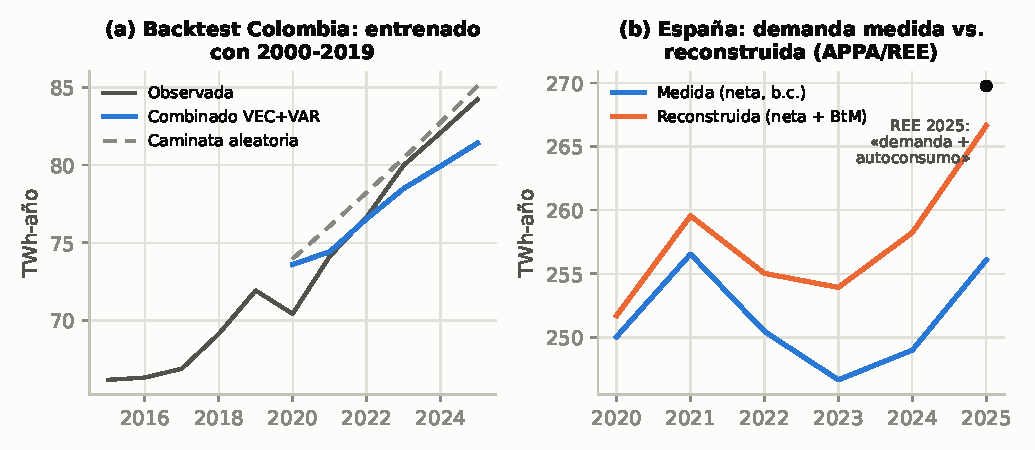
\includegraphics[width=.98\linewidth]{f7_validacion.pdf}
\caption{Marco de validación. (a)~Backtest para Colombia: pronóstico
2020-2025 con el modelo entrenado hasta 2019, frente a la demanda observada
y a la caminata aleatoria con deriva. (b)~España: demanda medida (neta,
b.c.) frente a la reconstruida (neta + autoconsumo aprovechado, APPA); el
punto negro es la serie ``demanda + autoconsumo'' que REE publicó por
primera vez para 2025 (269.753~GWh). Elaboración propia.}
\label{fig:valid}
\end{figure}

\subsection{Proyección ajustada 2026-2040 y umbral CREG}

La Figura~\ref{fig:proy} presenta el ajuste BtM sobre la demanda bruta
2026-2040: la demanda neta de 2040 quedó entre 136,1~TWh (E2) y 143,6~TWh
(E1), es decir, el BtM ``enmascararía'' entre 4,0 y 11,5~TWh-año en 2040 y
recortaría la TCAC 2025-2040 de 3,8\,\% a 3,2-3,6\,\%. La
Tabla~\ref{tab:umbral} resume las capacidades por escenario y los años de
cruce del umbral del 4\,\%: contabilizando toda la generación BtM (criterio
del cálculo CREG de 1,2~GW \cite{creg901099}), la senda tendencial de la
UPME lo cruza en 2029 y las sendas E2-E3 en 2030; contabilizando solo
excedentes del 40\,\%, los cruces se desplazan a 2034-2040. En potencia
máxima, el BtM fotovoltaico sin almacenamiento no reduce la punta nocturna
del SIN (${\sim}$19-20~h): bajo E2, la carga neta del mediodía de 2035 cae
${\sim}3{,}7$~GW con punta intacta (Anexo~D). El efecto sobre la energía
anual (3-8\,\% según escenario) no es proporcional al de potencia: el factor
de carga del SIN, $FC=D_{GWh}/(8760\cdot P_{max,MW})$, se deteriora porque
el denominador casi no cambia mientras el numerador sí, obligando a
remunerar la misma capacidad firme de generación y transporte sobre un
menor volumen de energía neta. El umbral del 4\,\% además se evalúa por
mercado de comercialización, no sobre el SIN agregado \cite{creg101072}; en
mercados de mayor irradiación y costo unitario, como los de la Costa Caribe
(Afinia, Air-e), es plausible que se alcance un par de años antes que el
promedio nacional aquí estimado, hacia 2027-2028, aunque una estimación
rigurosa exigiría desagregar el análisis por mercado, lo que queda como
trabajo futuro (Sección~6).

\begin{figure}[htb]\centering
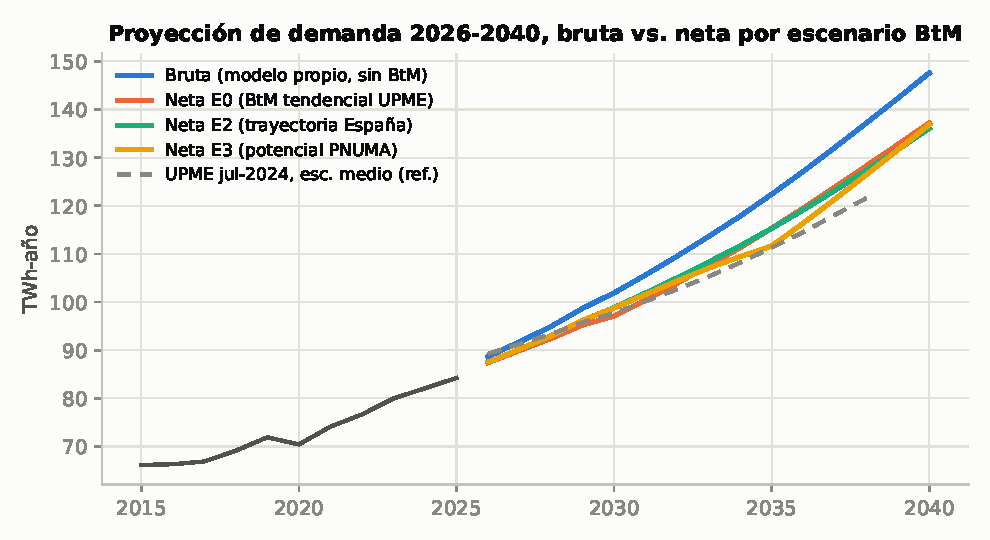
\includegraphics[width=.84\linewidth]{f2_proyeccion_escenarios.pdf}
\caption{Demanda histórica (XM) y proyección 2026-2040: bruta del modelo
propio frente a netas por escenario BtM, con la senda oficial UPME jul-2024
como referencia. Elaboración propia.}
\label{fig:proy}
\end{figure}

\begin{table}[htb]\centering\small
\caption{Escenarios BtM y cruce del umbral CREG del 4\,\% (energía BtM total
sobre demanda regulada; entre paréntesis, contabilizando solo excedentes
${\approx}40$\,\%).}
\label{tab:umbral}
\begin{tabular}{lrrrrc}
\toprule
Escenario & MW 2026 & MW 2030 & MW 2040 & \%MR 2030 & Cruce 4\,\%\\
\midrule
E0 Tendencial UPME & 896 & 3.331 & 7.182 & 7,0 & 2029 (2040)\\
E1 Envolvente CREG 4\,\% & 1.669 & 1.918 & 2.777 & 4,0 & no cruza\\
E2 Trayectoria España & 842 & 2.119 & 7.964 & 4,4 & 2030 (2038)\\
E3 Potencial PNUMA & 824 & 2.188 & 7.424 & 4,6 & 2030 (2034)\\
\bottomrule
\end{tabular}
\end{table}

% ============================================================ DISCUSION
\section{Discusión}

Los resultados de la validación sostienen las tres afirmaciones centrales
del trabajo. Primero, \emph{el enmascaramiento es real y medible}: en la
Figura~\ref{fig:valid}(b) la demanda española medida de 2025 apenas recupera
el nivel de 2021, mientras la reconstruida lo supera con holgura; APPA lo
formula sin rodeos al señalar que el autoconsumo ``se consideraba como una
disminución de la demanda, lo cual hacía que las cifras de consumo eléctrico
no estuvieran ajustadas a la realidad'' \cite{appa2025}; además, REE comenzó
en 2025 a publicar oficialmente la serie ``demanda + autoconsumo''
(269.753~GWh; crecimiento de 3,7\,\% frente a 2,8\,\% de la medida)
\cite{reeise}. Que el operador del sistema español haya institucionalizado
exactamente el Paso~1 aquí propuesto es, a juicio de los autores, la
validación externa más contundente de la metodología. Segundo, \emph{la
distorsión econométrica opera como predice la teoría}: el coeficiente del
panel (ec.~\ref{eq:panel}) es compatible con el enmascaramiento uno a uno
($p=0{,}30$ para $H_0\!:c=-1$), la elasticidad aparente española cae de 0,27
a 0,11 al usar demanda neta, y en Colombia bastó el quiebre de 2020 para
voltear el signo de $\alpha$ en el VECM (Tabla~\ref{tab:econ}b), el mismo
tipo de contaminación que el BtM produciría de forma permanente y creciente.
Tercero, \emph{el instrumento de pronóstico es competitivo}: el MAPE de
1,15\,\% del modelo combinado en 2022-2025 mejora los referentes
univariados y es del orden de los errores que reporta la UPME para sus
propios escenarios \cite{upme2024}; que ningún modelo supere a la caminata
aleatoria a través del choque de 2020 no es una falla del marco sino la
evidencia de que los quiebres de la serie medida son impredecibles desde la
propia serie; esta es una razón adicional para corregirla ex ante en lugar
de pronosticar sobre ella.

Frente a la senda oficial, la demanda bruta propia crece más rápido (TCAC
3,8\,\% vs.\ 2,99\,\% \cite{upme2026}), por la elasticidad estimada en el
ciclo expansivo 2021-2025 y por tomar la cuña GCE sin depurar
probabilidades de materialización; el diferencial bruta-neta (0,2-0,6
puntos de TCAC según escenario) es, en cambio, robusto al nivel de la línea
base y coherente con el punto porcentual que separa los propios escenarios
GD de la UPME \cite{upme2026}. Sobre el umbral del 4\,\%: no es un límite
físico sino una señal de revisión tarifaria; según su soporte técnico, con
${\sim}1{,}2$~GW en créditos de energía el costo unitario de nivel~1 subiría
${\sim}3{,}5$\,\% \cite{creg901099}. Además, resultará \emph{temprana}, pues
la propia senda tendencial de la UPME la cruza hacia 2029-2030. Comparado
con España, que alcanzó 4,1\,\% de cobertura sin colapso tarifario con
compensación de excedentes a precio de mercado, el 4\,\% colombiano es restrictivo como señal de largo
plazo pero apunta en la dirección correcta tras la reforma del art.~12
(remuneración referenciada a MC) \cite{creg101072}; el error sería tratarlo
como tope de planeación, pues todos los escenarios lo desbordan y no captura
ni los autoconsumos instantáneos ni el problema de potencia. La punta
nocturna no se reduce, como lo confirma España con 9.590~MW BtM y punta
anual intacta \cite{ree2026}; el almacenamiento BtM, que allí creció 119\,\%
tras el apagón de abril de 2025 \cite{appa2025}, es el complemento que sí
desplaza punta.

La proyección de demanda no es un ejercicio aislado, alimenta directamente
el dimensionamiento de la expansión de transmisión. El Plan de Expansión de
Referencia Generación-Transmisión \cite{plangt2016} refuerza el STN y los
STR para cumplir el criterio de confiabilidad N-1 precisamente en las horas
de mayor exigencia del sistema, que en Colombia siguen siendo las nocturnas.
Si la UPME dimensiona o posterga esas obras a partir de una demanda neta ya
enmascarada por el BtM, arriesga subestimar la capacidad de transporte que
la red seguirá necesitando en la punta, pues, como se mostró arriba, el BtM
solar no la alivia. A esto se suma un desafío técnico distinto al de
energía: los flujos bidireccionales al mediodía en nodos con alta
concentración solar, como los de la Costa Caribe y el Valle del Cauca,
exigen capacidad de transformación AT/MT dimensionada para exportar y no
solo para importar, un problema de potencia que la proyección agregada de
energía anual no captura. Como limitaciones: las muestras anuales son cortas (el IC
del panel es amplio y la cointegración es sensible a la determinística), el
estimador de reconstrucción pierde precisión en fases tempranas de adopción
(errores de 30-40\,\% en España 2019-2021) y el factor de planta se trató
como constante; nada de ello altera las conclusiones cualitativas, pero
acota la precisión numérica de los cruces del umbral ($\pm1$~año ante
$FC\in[15;18]$\,\%).

% ========================================================= CONCLUSIONES
\section{Conclusiones}

Este trabajo se propuso incorporar el efecto BtM en la estimación de demanda
de largo plazo del sistema colombiano y, como lo exige el método científico,
probar la propuesta con datos históricos. La metodología de cuatro pasos, que consiste en reconstruir la demanda bruta
desde el registro de capacidad, estimar la combinación VAR/VEC sobre ella,
proyectar la adopción BtM con escenarios exógenos y publicar siempre la
pareja bruta/neta, superó las tres pruebas
planteadas: el \emph{backtest} colombiano arrojó un MAPE de 1,15\,\% frente
a 1,79-2,36\,\% de los referentes univariados; el experimento español
demostró que el 60\,\% del crecimiento real del consumo 2020-2025 quedó
oculto al sistema de medida y que el estimador de reconstrucción reproduce
la generación BtM con errores menores al 3\,\% una vez maduro el registro; y
el panel binacional no rechazó el enmascaramiento uno a uno que predice la
teoría ($\hat{c}=-3{,}1$; $p=0{,}30$ para $c=-1$). Aplicada a 2026-2040, la
metodología cuantifica una demanda enmascarada de 4,0 a 11,5~TWh-año en 2040
(0,2-0,6 puntos de TCAC) y muestra que el BtM fotovoltaico no reduce la
punta nocturna del SIN: reconfigura la curva de carga, con un hueco solar de
${\sim}3{,}7$~GW al mediodía de 2035 y rampas vespertinas mayores.

De estos resultados se desprenden tres recomendaciones. La UPME debería
institucionalizar la reconstrucción de demanda bruta como paso previo a la
estimación, apoyada en un registro de instalaciones BtM completo y oportuno;
el precedente de REE, que ya publica la serie de demanda más autoconsumo,
muestra el camino, y la debilidad de un registro incompleto fue el costo que
España pagó caro. La
CREG debería tratar el umbral del 4\,\% como lo que es, una señal de
revisión tarifaria que se activará temprano (2029-2034 según escenario y
contabilización), y evolucionar hacia una senda explícita de integración, con remuneración
eficiente de excedentes, cargos de red por capacidad y señales horarias,
antes de que el umbral se vuelva vinculante. Y la
planeación de potencia, incluida la expansión de transmisión del Plan GT
\cite{plangt2016}, debe dimensionarse sobre la demanda bruta y no sobre la
neta enmascarada, modelar el BtM como cambio de forma de la curva de carga y
valorar el almacenamiento detrás del contador como el complemento que sí
desplaza punta. Como trabajo futuro se recomienda desagregar el análisis por
mercado de comercialización, comenzando por los de mayor irradiación y costo
unitario como los de la Costa Caribe, cuando el registro AGPE acumule
historia suficiente; incorporar el precio minorista al sistema VEC; y
modelar horariamente el hueco solar con los perfiles de XM. Las limitaciones
de muestra y de calibración señaladas en la discusión acotan la precisión,
no la dirección, de los hallazgos.

% ========================================================== REFERENCIAS
\begingroup
\small
\begin{thebibliography}{99}\setlength{\itemsep}{1pt}

\bibitem{upme2026} UPME. \emph{Proyección de la demanda de energía eléctrica y
potencia máxima 2026-2040}, revisión julio 2026. Bogotá, 2026.

\bibitem{appa2025} APPA Renovables. \emph{Informe anual del autoconsumo
fotovoltaico y almacenamiento 2025}. Madrid, 2026.

\bibitem{ree2026} Red Eléctrica de España. \emph{Máximos anuales de demanda},
sistemaelectrico-ree.es, consulta agosto 2026.

\bibitem{reeise} Red Eléctrica de España. \emph{El sistema eléctrico español
2025} (informe y nota de prensa, marzo 2026). Madrid, 2026.

\bibitem{proyecto} ILE4100. \emph{Proyecto 1, Planeamiento de Sistemas de
Potencia} (enunciado). Universidad de los Andes, 2026.

\bibitem{upmetechos} UPME. ``Colombia supera los 24.000 techos solares y
acelera la democratización de la energía limpia''. Noticia, 13 de mayo de 2026.

\bibitem{pnuma2021} PNUMA. \emph{La oportunidad de negocio de la Generación
Solar Distribuida en Colombia}. Bogotá, 2021.

\bibitem{creg101072} CREG. \emph{Resolución 101~072 de 2025}: integración de
las comunidades energéticas (AGRC y GDC) al SIN y a las ZNI. Art.~12.

\bibitem{creg901099} CREG. \emph{Documento CREG 901~099 de 2024: Comunidades
Energéticas} (soporte del proyecto de Res.\ 701~051 de 2024). Sesión 1322.

\bibitem{creg174} CREG. \emph{Resolución 174 de 2021}: autogeneración a
pequeña escala y generación distribuida en el SIN.

\bibitem{upme2024} UPME. \emph{Proyección de la demanda de energía eléctrica y
potencia máxima 2024-2038}, revisión julio 2024. Bogotá, 2024.

\bibitem{upmeene2026} UPME. \emph{Proyección de la demanda de energía
eléctrica y potencia máxima 2025-2039}, revisión enero 2026. Bogotá, 2026.

\bibitem{upme2021} UPME. \emph{Proyección de demanda de energía eléctrica},
revisión junio 2021. Bogotá, 2021.

\bibitem{plangt2016} UPME. \emph{Plan de Expansión de Referencia
Generación-Transmisión 2016-2030}. Bogotá, 2016.

\bibitem{vargas2025} Vargas-Forero, V., Manotas-Duque, D. y Trujillo, L.
``Comparative study of forecasting methods to predict the energy demand for
the market of Colombia''. \emph{Int.\ J.\ of Energy Economics and Policy},
15(1), 65-76, 2025.

\bibitem{grimaldo2021} Grimaldo-Guerrero, J. et al. ``The behavior of the
annual electricity demand and the role of economic growth in Colombia''.
\emph{IJEEP}, 11(5), 8-12, 2021.

\bibitem{gujarati} Gujarati, D. y Porter, D. \emph{Econometría}, 5.ª ed.
McGraw-Hill, 2010. Caps.\ 16, 21 y 22.

\bibitem{castano1994} Castaño, E. ``Combinación de pronósticos y variables
predictoras con error''. \emph{Lecturas de Economía}, 41, 59-80, 1994.

\bibitem{masih1996} Masih, R. y Masih, A. ``Stock-Watson dynamic OLS (DOLS)
and error-correction modelling approaches to estimating long- and short-run
elasticities in a demand function''. \emph{Energy Economics}, 18(4), 1996.

\bibitem{engle1987} Engle, R. y Granger, C. ``Co-integration and error
correction''. \emph{Econometrica}, 55(2), 251-276, 1987.

\bibitem{johansen1988} Johansen, S. ``Statistical analysis of cointegration
vectors''. \emph{J.\ of Economic Dynamics and Control}, 12, 231-254, 1988.

\bibitem{sims1980} Sims, C. ``Macroeconomics and reality''.
\emph{Econometrica}, 48(1), 1-48, 1980.

\bibitem{xm2025} XM. ``En 2024, la demanda de energía en Colombia aumentó
2,3\,\%'' (82.084,9~GWh). Comunicado, enero 2025.

\bibitem{xm2026} La República / XM. ``La demanda de energía eléctrica del SIN
creció 2,62\,\% en 2025''. Enero 2026.

\bibitem{sercol2026} SER Colombia. \emph{Balance renovable 2026: 4.000~MW
proyectados}. Bogotá, febrero 2026.

\end{thebibliography}
\endgroup

\clearpage
\appendix
% ================================================================ ANEXOS
\renewcommand{\thesection}{Anexo \Alph{section}}
\renewcommand{\thesubsection}{\Alph{section}.\arabic{subsection}}
\setcounter{section}{0}
\setcounter{table}{0}\renewcommand{\thetable}{A\arabic{table}}
\setcounter{figure}{0}\renewcommand{\thefigure}{A\arabic{figure}}

\begin{center}
{\Large\bfseries Anexos}\\[2pt]
{\small (material complementario; máximo 20 páginas)}
\end{center}

% ------------------------------------------------------------------ A
\section{Repositorio GitHub con los códigos fuente}
\label{anexo:repo}

Todo el análisis es reproducible desde el repositorio del grupo:

\begin{center}
\fbox{\parbox{.86\linewidth}{\centering\ttfamily
https://github.com/$\langle$usuario$\rangle$/proyecto1-btm-demanda\\[2pt]
\footnotesize (actualizar con el enlace definitivo al publicar; ver instrucciones abajo)}}
\end{center}

\subsection{Estructura}
\begin{verbatim}
proyecto1-btm-demanda/
|- README.md                  <- documentacion y guia de reproduccion
|- requirements.txt           <- numpy, pandas, statsmodels, matplotlib
|- data/
|  |- demanda_pib_anual.csv   <- demanda SIN (GWh) y PIB real, 2000-2025
|  |- upme_proyeccion_jul2024.csv <- proyeccion oficial UPME (esc. medio)
|  |- espana_anual.csv        <- demanda b.c., autoconsumo y PIB de Espana
|  |- parametros_btm.csv      <- parametros con fuente (CREG, APPA, PNUMA...)
|- src/
|  |- config.py               <- rutas, paleta de figuras y supuestos
|  |- analisis_econometrico.py<- ADF/KPSS, Johansen, Engle-Granger,
|  |                             VECM, VAR, combinacion de pronosticos
|  |- ajuste_btm.py           <- demanda bruta y escenarios BtM E0-E3
|  |- validacion.py           <- V1 backtest, V2 experimento Espana,
|  |                             V3 panel LSDV Colombia-Espana
|  |- generar_figuras.py      <- figuras F1-F7 del informe
|  |- descargar_datos.py      <- refresco opcional desde XM (pydataxm),
|  |                             Banco Mundial y anexo Excel UPME 2026-2040
|- output/                    <- tablas CSV y figuras (se regeneran)
|- informe/                   <- fuentes LaTeX de este documento
\end{verbatim}

\subsection{Reproducción}
\begin{verbatim}
pip install -r requirements.txt
cd src
python analisis_econometrico.py   # econometria y proyeccion organica
python ajuste_btm.py              # escenarios BtM y demanda neta
python validacion.py              # V1 backtest, V2 Espana, V3 panel
python generar_figuras.py         # figuras
\end{verbatim}
Los cuatro scripts corren en menos de un minuto y regeneran todas las tablas
y figuras de este informe. Para publicar el repositorio desde la cuenta de un
integrante: \texttt{git init \&\& git add .\ \&\& git commit}, crear el
repositorio vacío en GitHub y \texttt{git push -u origin main}.

% ------------------------------------------------------------------ B
\section{Resultados econométricos completos}

\subsection{Cointegración de Johansen (sensibilidad a muestra y determinística)}

\begin{table}[htb]\centering\small
\caption{Prueba de la traza de Johansen, $H_0\!: r=0$ vs.\ $r\le1$
($k=1$ rezago en diferencias).}
\begin{tabular}{llcccc}
\toprule
Determinística & Muestra & Traza $r{=}0$ & VC 90\,\% & VC 95\,\% & ¿Rechaza 95\,\%?\\
\midrule
Constante            & 2000-2025 & 3,87  & 13,43 & 15,49 & No\\
Constante            & 2000-2019 & 4,64  & 13,43 & 15,49 & No\\
Constante+tendencia  & 2000-2025 & 10,57 & 16,16 & 18,40 & No\\
Constante+tendencia  & 2000-2019 & \textbf{19,88} & 16,16 & 18,40 & \textbf{Sí}\\
\bottomrule
\end{tabular}
\end{table}

Complemento de Engle-Granger (2000-2025): regresión estática
$\ln D_t = 1{,}030 + 0{,}742\,\ln Y_t$ ($R^2=0{,}985$); ADF sobre los
residuos $=-2{,}55$ ($p\approx0{,}0105$): se rechaza no cointegración al
5\,\%. La evidencia conjunta respalda una relación de largo plazo, cuya
inferencia se debilita con el quiebre de 2020, el mismo mecanismo que el BtM
reproducirá de forma permanente sobre la demanda medida.

\subsection{Combinación de pronósticos}

Ponderaciones por inverso del error cuadrático medio de pronósticos a un paso
en evaluación pseudo-fuera-de-muestra 2015-2025 (reestimación recursiva):
VEC 0,456; VAR(1) en diferencias 0,544. El procedimiento replica, a escala,
el esquema oficial (Tabla~1 del informe). Proyección resultante del SIN
orgánico y demanda bruta (con cuña incremental GCE+ME de la UPME):

\begin{table}[htb]\centering\small
\caption{Proyección propia 2026-2040 (GWh-año, escenario medio).}
\begin{tabular}{lrrrrr}
\toprule
 & 2026 & 2030 & 2035 & 2038 & 2040\\
\midrule
SIN orgánico (modelo)        & 86.879 & 98.248 & 114.569 & 125.633 & 133.595\\
Cuña incremental GCE+ME      & 1.829  & 3.661  & 7.820   & 11.520  & 13.987\\
\textbf{Demanda bruta}       & \textbf{88.708} & \textbf{101.909} & \textbf{122.389} & \textbf{137.153} & \textbf{147.582}\\
Referencia UPME jul-2024 (SIN+GCE+ME+GD) & 89.253 & 97.682 & 111.295 & 121.569 & n.d.\\
\bottomrule
\end{tabular}
\end{table}

La senda propia crece más rápido que la referencia oficial (TCAC 3,8\,\% vs.\
2,99\,\% de la rev.\ jul-2026) por dos razones: la elasticidad estimada en la
muestra completa (0,75) recoge el ciclo expansivo 2021-2025, y la cuña GCE se
toma del reporte oficial sin depurar probabilidades de materialización. Para
efectos del análisis BtM lo relevante es el \emph{diferencial} bruta-neta,
que es robusto al nivel de la línea base.

\subsection{Marco de validación: resultados completos}

\begin{table}[htb]\centering\small
\caption{V1. Backtest retrospectivo en Colombia: pronóstico condicional al
PIB observado, por corte de entrenamiento y modelo.}
\begin{tabular}{clcc}
\toprule
Entrenamiento & Modelo & MAPE (\%) & RMSE (GWh)\\
\midrule
\multirow{3}{*}{2000-2019 (pron.\ 2020-2025)}
 & Combinado VEC+VAR & 2,15 & 2.043\\
 & Caminata aleatoria c/deriva & 2,02 & 1.835\\
 & AR(1) univariado & 2,47 & 2.097\\
\midrule
\multirow{3}{*}{2000-2021 (pron.\ 2022-2025)}
 & Combinado VEC+VAR & \textbf{1,15} & \textbf{1.235}\\
 & Caminata aleatoria c/deriva & 1,79 & 1.552\\
 & AR(1) univariado & 2,36 & 1.983\\
\bottomrule
\end{tabular}
\end{table}

\begin{table}[htb]\centering\small
\caption{V2. España: validación del estimador de reconstrucción del
Paso~1. Horas equivalentes calibradas únicamente con 2025
($h=1.174$~h-año); generación estimada
$\widehat{G}_t=\bar{P}_t\cdot h$ vs.\ real (APPA).}
\begin{tabular}{lrrr}
\toprule
Año & $\widehat{G}$ estimada (GWh) & $G$ real (GWh) & Error (\%)\\
\midrule
2019 & 554   & 925    & $-40{,}1$\\
2020 & 1.095 & 1.656  & $-33{,}9$\\
2021 & 2.100 & 3.007  & $-30{,}2$\\
2022 & 4.442 & 4.564  & $-2{,}7$\\
2023 & 7.261 & 7.262  & $0{,}0$\\
2024 & 9.120 & 9.243  & $-1{,}3$\\
2025 & 10.550 & 10.550 & (calibración)\\
\bottomrule
\end{tabular}
\end{table}

\begin{table}[htb]\centering\small
\caption{V3. Panel Colombia-España en tasas de crecimiento (LSDV,
ec.~4 del informe), errores estándar robustos HC1.}
\begin{tabular}{lc}
\toprule
Parámetro & Valor\\
\midrule
$\hat{c}$ (coeficiente de $\Delta s$ BtM) & $-3{,}079$\\
Error estándar robusto & 1,960\\
IC 95\,\% & $[-6{,}92;\ 0{,}76]$\\
$t$ de $H_0\!:c=-1$ ($p$-valor) & $-1{,}06$ (0,299)\\
Elasticidad PIB de corto plazo, Colombia & 0,226\\
Elasticidad PIB de corto plazo, España (demanda neta) & $-0{,}236$\\
$R^2$ / observaciones & 0,58 / 30\\
\bottomrule
\end{tabular}
\end{table}

Notas metodológicas de V3: en niveles, $s_t$ y $\ln Y_t$ resultan casi
colineales en la corta muestra española (2020-2025) y el coeficiente $c$ no
queda identificado (el ejercicio en niveles arroja signos inestables); por
ello la especificación se planteó en primeras diferencias, donde la variación
de instalación anual $\Delta s$ se separa del ciclo del PIB. La elasticidad
española de corto plazo negativa sobre demanda \emph{neta} es en sí misma
sintomática del enmascaramiento que el término $\Delta s$ corrige. La serie
de participación colombiana usa el registro de capacidad AGPE/GD (235,66~MW
acumulados a 2023 y 339~MW a 2024, según UPME; 645~MW a 2025, rev.\
ene-2026), con generación a factor de planta de 16,5\,\%.

% ------------------------------------------------------------------ C
\section{Escenarios BtM año a año}

\begin{table}[htb]\centering\small
\caption{Capacidad BtM instalada por escenario (MW).}
\begin{tabular}{lrrrr}
\toprule
Año & E0 UPME & E1 CREG 4\,\% & E2 España & E3 PNUMA\\
\midrule
2026 & 896   & 1.669 & 842   & 824\\
2028 & 1.727 & 1.787 & 1.365 & 1.342\\
2030 & 3.331 & 1.918 & 2.119 & 2.188\\
2032 & 3.884 & 2.061 & 3.107 & 3.567\\
2034 & 4.529 & 2.217 & 4.276 & 5.815\\
2035 & 4.891 & 2.303 & 4.903 & 7.424\\
2036 & 5.282 & 2.392 & 5.539 & 7.424\\
2038 & 6.159 & 2.581 & 6.794 & 7.424\\
2040 & 7.182 & 2.777 & 7.964 & 7.424\\
\bottomrule
\end{tabular}
\end{table}

\begin{table}[htb]\centering\small
\caption{Demanda neta por escenario (GWh-año) y energía enmascarada en 2040.}
\begin{tabular}{lrrrrr}
\toprule
Trayectoria & 2030 & 2035 & 2040 & TCAC 25-40 & Enmascarado 2040\\
\midrule
Demanda bruta (sin BtM) & 101.909 & 122.389 & 147.582 & 3,81\,\% & 0\\
Neta E0 (tendencial UPME) & 97.094 & 115.320 & 137.201 & 3,31\,\% & 10.381\\
Neta E1 (envolvente CREG) & 99.137 & 119.060 & 143.568 & 3,62\,\% & 4.014\\
Neta E2 (trayectoria España) & 98.846 & 115.302 & 136.071 & 3,25\,\% & 11.511\\
Neta E3 (potencial PNUMA) & 98.746 & 111.658 & 136.851 & 3,29\,\% & 10.731\\
\bottomrule
\end{tabular}
\end{table}

Supuestos: factor de planta FV 16,5\,\% (1~MW $\to$ 1,445~GWh-año;
sensibilidad 15-18\,\% desplaza los cruces del umbral $\pm1$ año);
participación del mercado regulado 68\,\% de la demanda comercial; en E1 se
computa toda la generación BtM contra el umbral (interpretación del cálculo
CREG de 1,2~GW $\leftrightarrow$ 4\,\%); la contabilización alternativa con
excedentes del 40\,\% se reporta en la Tabla~3 del informe.

\begin{figure}[htb]\centering
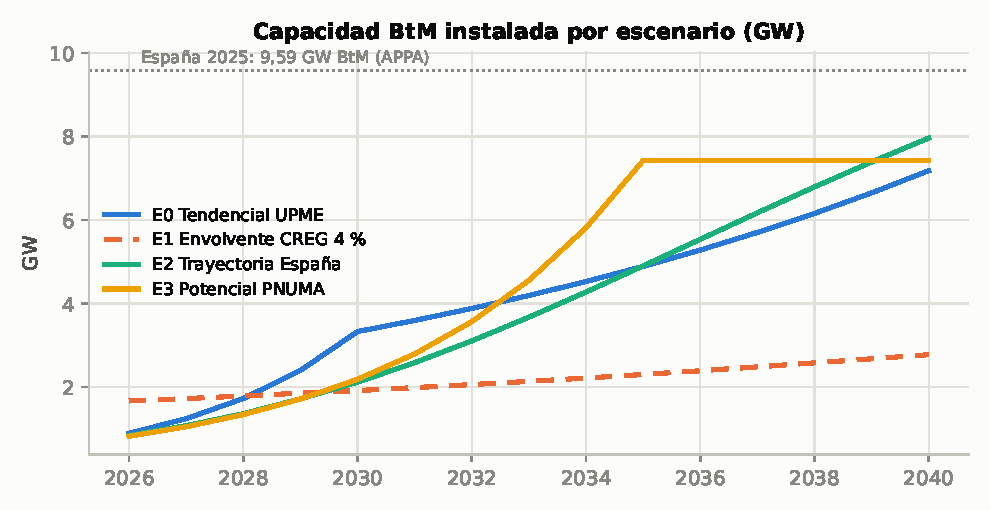
\includegraphics[width=.8\linewidth]{f3_capacidad_btm.pdf}
\caption{Capacidad BtM por escenario y referencia de España (9,59~GW a 2025).
Elaboración propia.}
\end{figure}

% ------------------------------------------------------------------ D
\section{Figuras complementarias}

\begin{figure}[htb]\centering
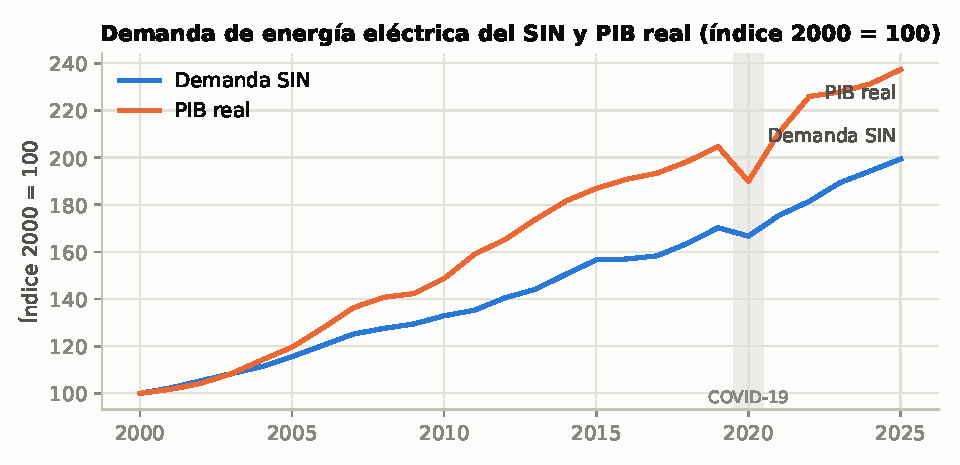
\includegraphics[width=.78\linewidth]{f1_demanda_pib.pdf}
\caption{Demanda del SIN y PIB real de Colombia, índice 2000=100. La demanda
crece por debajo del PIB (elasticidad $<1$) y el choque de 2020 rompe
transitoriamente la relación. Fuentes: XM, DANE/Banco Mundial.}
\end{figure}

\begin{figure}[htb]\centering
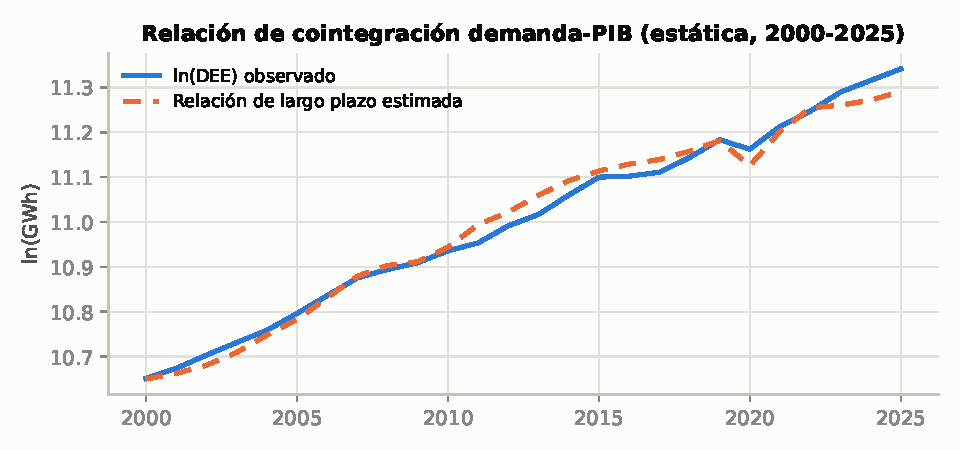
\includegraphics[width=.78\linewidth]{f6_cointegracion.pdf}
\caption{Relación de cointegración estática $\ln D$-$\ln Y$ (2000-2025).}
\end{figure}

\begin{figure}[htb]\centering
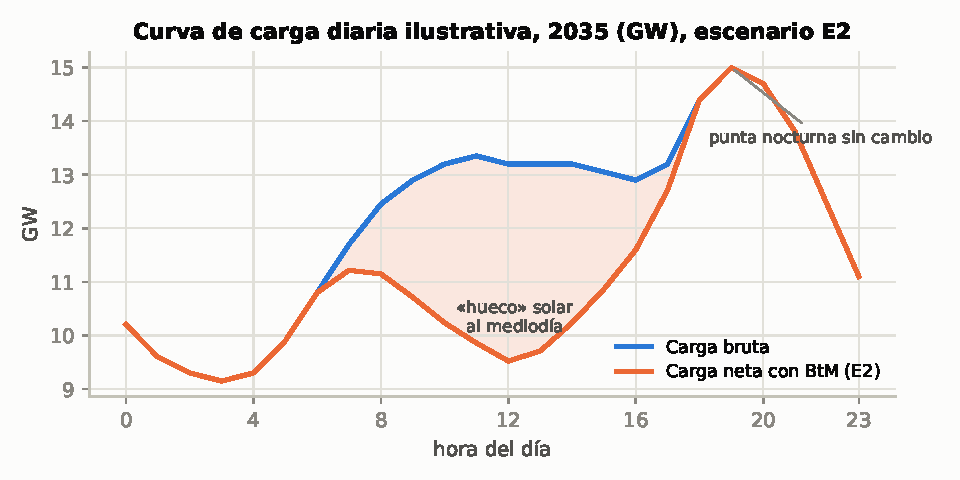
\includegraphics[width=.8\linewidth]{f5_curva_carga.pdf}
\caption{Curva de carga diaria ilustrativa a 2035 bajo E2 (forma típica de
día hábil del SIN, punta nocturna normalizada a la potencia máxima proyectada).
El BtM fotovoltaico deprime el mediodía (${\sim}3{,}7$~GW) sin tocar la punta
de las 19-20~h: el fenómeno de la ``curva de pato''. Elaboración propia.}
\end{figure}

\begin{figure}[htb]\centering
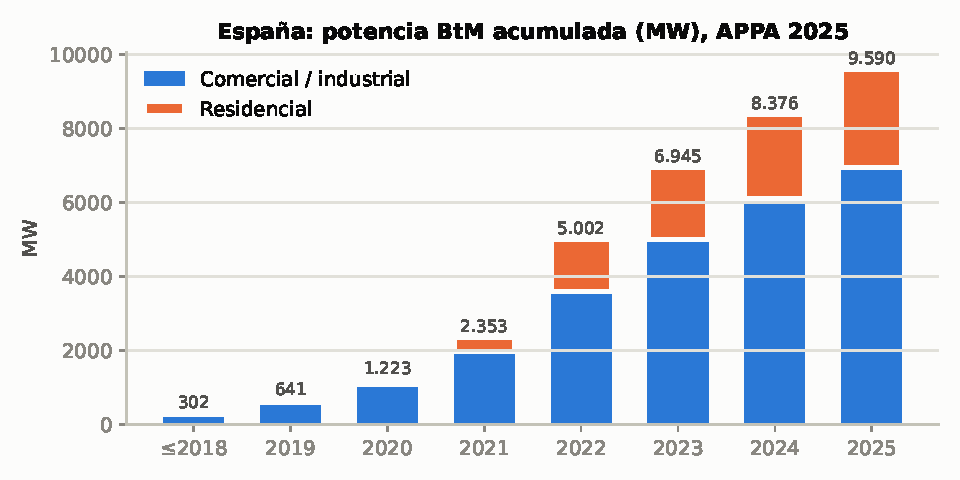
\includegraphics[width=.8\linewidth]{f4_espana_btm.pdf}
\caption{España: potencia BtM acumulada por segmento, 2018-2025 (APPA).
De 302~MW a 9.590~MW en ocho años; el segmento comercial/industrial domina.}
\end{figure}

% ------------------------------------------------------------------ E
\section{Material complementario: regulación y caso España}

\subsection{Marco regulatorio colombiano del BtM}

\begin{itemize}
\item \textbf{Ley 1715 de 2014} (mod.\ Ley 2099 de 2021): promueve FNCER,
autogeneración y entrega de excedentes.
\item \textbf{Res.\ CREG 030 de 2018 $\to$ 174 de 2021}: reglas de AGPE
($\le1$~MW... hasta 5~MW para autogeneración a pequeña escala según ajustes
posteriores) y GD ($<1$~MW en SDL); créditos de energía: excedentes tipo~1
(hasta el consumo) valorados a costo de compra del comercializador, tipo~2 a
precio de bolsa.
\item \textbf{Ley 2294 de 2023 (art.\ 235) y Decreto 2236 de 2023}: crean las
\emph{comunidades energéticas} (AGRC y GDC).
\item \textbf{Doc.\ CREG 901~099 de 2024}: soporte técnico; simula que con
1,2~GW de autogeneración con créditos (equivalente al 4\,\% de la energía del
mercado regulado) el costo unitario de nivel de tensión~1 sube
${\sim}3{,}5$\,\% si todos los excedentes son tipo~1.
\item \textbf{Res.\ CREG 101~072 de 2025 (art.\ 12)}: versión definitiva;
umbral de revisión del 4\,\% de la demanda comercial regulada por mercado de
comercialización; remuneración de excedentes referenciada a MC (precio medio
de contratos del mercado regulado) para estabilizar la señal de precio.
\item \textbf{Contexto de expansión}: el Plan 6GW+ y el balance gremial 2026
(${\sim}4.000$~MW renovables proyectados, de los cuales ${\sim}1.300$~MW en
recursos distribuidos) aceleran la base instalada BtM.
\end{itemize}

\subsection{Indicadores del caso español (APPA 2025 y REE)}

\begin{table}[htb]\centering\small
\caption{España: indicadores BtM 2025.}
\begin{tabular}{lr}
\toprule
Potencia BtM acumulada & 9.590~MW\\
Nueva potencia 2025 (residencial / C\&I) & 1.214~MW (368 / 846)\\
Generación BtM aprovechada 2025 & 10.550~GWh\\
Generación no aprovechada (vertidos limitados) & 2.183~GWh\\
Cobertura de la demanda nacional (256.085~GWh) & 4,1\,\%\\
Punta anual del sistema (15-ene-2025, 20:57) & 40.070~MW\\
Almacenamiento BtM instalado en 2025 & 339~MWh ($+119$\,\%)\\
``Demanda + autoconsumo'' publicada por REE (2025) & 269.753~GWh ($+3{,}7$\,\%)\\
\bottomrule
\end{tabular}
\end{table}

Series anuales empleadas en la validación (APPA, figuras 8, 10 y 11 del
informe): producción de autoconsumo aprovechada 2018-2025 de 446, 925,
1.656, 3.007, 4.564, 7.262, 9.243 y 10.550~GWh; demanda nacional b.c.\
2020-2025 de 250.051, 256.546, 250.471, 246.665, 249.000 y 256.085~GWh; y
energía no aprovechada 2018-2025 de 120, 249, 431, 749, 1.384, 1.899, 2.094
y 2.183~GWh.

Lecciones para Colombia: (i)~la adopción es no lineal y dominada por el
segmento comercial-industrial; (ii)~la cobertura energética del 4\,\% se
alcanzó en ${\sim}7$ años desde el despegue regulatorio (RD 244/2019);
(iii)~la punta del sistema no se redujo, pues el valor de capacidad del BtM
fotovoltaico es bajo sin almacenamiento; (iv)~el evento de ``cero
energético'' de abril de 2025 disparó el almacenamiento detrás del contador
(+119\,\%), añadiendo un servicio de resiliencia que la regulación colombiana
aún no valora; y (v)~la falta de un registro oficial completo de
instalaciones es la principal debilidad estadística señalada por el sector;
Colombia puede evitarla fortaleciendo desde ya los reportes de la
Res.~CREG 174 de 2021 y el registro AGPE de la UPME, insumo directo del
Paso~1 de la metodología propuesta.

\subsection{Sobre los datos}

Demanda SIN 2017-2025 verificada contra XM (2024: 82.084,9~GWh; 2025
estimado con el crecimiento oficial de 2,62\,\%); 2000-2016 compilada de los
informes anuales de XM y regenerable con \texttt{descargar\_datos.py}
(API pydataxm). PIB real de Colombia y España en moneda constante de 2015
del Banco Mundial (serie NY.GDP.MKTP.KN, consistente con DANE e INE). La
proyección oficial UPME jul-2024 se transcribió del documento del curso; de
la rev.\ jul-2026 se tomaron las tasas de crecimiento y las anclas de GD
(3.331~MW a 2030 y 7.182~MW a 2040) publicadas por la UPME. Las series
españolas de la validación provienen del informe APPA 2025 del material del
curso y de REE (nota de prensa del sistema eléctrico 2025, que introduce la
serie oficial ``demanda + autoconsumo'': 269.753~GWh).

% ------------------------------------------------------------------ F
\section{Código fuente principal (extracto)}

Extracto de \texttt{src/ajuste\_btm.py} con la construcción de los
escenarios; el repositorio contiene el código completo comentado.

\begingroup\footnotesize
\begin{verbatim}
GWH_POR_MW = 8760 * FACTOR_PLANTA_FV / 1000.0   # ~1,45 GWh-anio por MW

def esc_tendencial_upme():
    """E0: anclas UPME rev. jul-2026 (645 MW en 2025, rev. ene-2026)."""
    return interp_geometrica({2025: 645, 2030: 3331, 2040: 7182}).loc[H]

def esc_creg_4pct(bruta):
    """E1: capacidad cuya generacion anual equivale al 4 % de la
    demanda comercial regulada (interpretacion conservadora art. 12)."""
    mr = PART_REGULADO * bruta["demanda_bruta_gwh"]
    return (UMBRAL_CREG * mr / GWH_POR_MW)

def esc_espana(bruta):
    """E2: la participacion BtM sobre demanda replica la senda
    espanola: 4,1 % al septimo anio del despegue; logistica s_max=9 %."""
    s_max, s_2025, s_2032 = 0.09, 0.011, 0.041
    def inv(s): return np.log(s_max / s - 1.0)
    k  = (inv(s_2025) - inv(s_2032)) / (2032 - 2025)
    t0 = 2025 + inv(s_2025) / k
    s  = s_max / (1.0 + np.exp(-k * (np.array(H) - t0)))
    return pd.Series(s * bruta["demanda_bruta_gwh"].values / GWH_POR_MW,
                     index=H)

def esc_pnuma():
    """E3: potencial de mercado PNUMA (7.424 MWp) alcanzado en 2035."""
    return interp_geometrica({2025: 645, 2035: 7424, 2040: 7424}).loc[H]

# demanda neta y umbral CREG
for e in ["E0_upme", "E1_creg4", "E2_espana", "E3_pnuma"]:
    gen = esc[f"{e}_mw"] * GWH_POR_MW
    res[f"{e}_neta_gwh"] = bruta["demanda_bruta_gwh"] - gen
    res[f"{e}_pct_umbral_total"] = 100 * gen / mr             # 100 % entregado
    res[f"{e}_pct_umbral_fe"] = 100 * 0.40 * gen / mr         # excedentes 40 %
\end{verbatim}
\endgroup


\end{document}
